\section{Modelling the shear correlation functions}
\label{sec:xipm}
A convenient way to infer cosmological information from observational data are the shear correlation functions $\xi_\pm$, which are defined as \[
\xi_\pm = \la \gamma_{\rm t}\gamma_{\rm t}\ra \pm \la \gamma_\times\gamma_\times\ra \, .
\]
They are the prime estimators to quantify a cosmic-shear signal since it is simple to include a weighting of the shear-measurements into the correlation functions and, contrary to the power spectrum, one does not have to worry about the shape of the survey footprint, or masked regions. Cosmologically, given two comoving distance probability distributions of sources $p_i(\chi),p_j(\chi)$, one can compute the shear correlation function from the underlyting matter power spectrum $P_\delta$ via \todo{Citation!}\begin{align}
\label{eq:xipm-pkappa}
\xi_\pm[\theta,p_i,p_j] =& \int_0^\infty \frac{{\rm d}l\,l}{2\pi}J_{0,4}(l\theta)P(l,p_i,p_j)\, , \\
\label{eq:pkappa-pdelta/lenseff}
P(l,p_i,p_j) =& \frac{9 H_0^4\Omega_{\rm m}^2}{4c^4}\int_0^{\chi_h} {\rm d}\chi\frac{g(\chi,p_i)g(\chi,p_j)}{a^2(\chi)}P_\delta\left(\frac{l}{f_K(\chi)},\chi\right)\, , \\
\label{eq:lenseff}
g(\chi,p_i) =& \int_\chi^{\chi_H} {\rm d}\chi'\, p_i(\chi') \frac{f_K(\chi'-\chi)}{f_K(\chi')}\, .
\end{align}
Here, $J_{0,4}$ denote the 0-th and 4-th order Bessel Functions.
\subsection{Using an analytic Model}
For a first simple analysis we will assume that a deeper redshift distribution just yields a stronger shear signal. Following \citet{2006APh....26...91V}, we estimate
\[
\la |\gamma| \ra \propto \la z \ra ^{0.85}\, .
\]
\todo{Maybe implement redshift-dependent index?}
Additionally, we assume that a higher depth does not only lead to a stronger average shear, but also to a higher galaxy number density, implying a correlation between those two quantities.

%For a pair of galaxies that we use to measure the correlation function, it is crucial to determine whether those two galaxies lie within the same pointing. We want to define a function $E(\theta)$ that determines 

Let $N(\b \theta)$ be the number-density per tile and $W(\b \theta)$ the weighting of average shear. The observed correlation function $\xi^{\text{obs}}_\pm(\theta)$ now changes from one of constant depth $\xi_\pm^{\rm const}$ via 
\begin{align*}
\xi^{\text{obs}}_\pm(\theta) = & \frac{\la N(\b 0)N(\b \theta)\gammao_{\rm t}(\b 0)\gammao_{\rm t}(\b \theta)\ra }{\la N(\b 0)N(\b \theta)\ra} \pm \frac{\la N(\b 0)N(\b \theta)\gammao_\times(\b 0)\gammao_\times(\b \theta)\ra }{\la N(\b 0)N(\b \theta)\ra} \\
 = & \frac{\la N(\b 0)N(\b \theta)W(\b 0)W(\b \theta)\ra}{\la N(\b 0)N(\b \theta)\ra} \xi_{\pm}^{\rm const}(\theta) \, .
 \end{align*}
 Assuming that depth and galaxy number density of neighbouring pointings are uncorrelated, the only important property of a galaxy pair is whether or not they lie in the same pointing. We want to denote the probability that a random pair of galaxies of distance $\theta$ lie in the same pointing with $E(\theta)$. An analytical expression for this function is surprisingly hard to obtain, but it can easily be calculated to arbitrary accuracy, following the procedure explained in Appendix \ref{sec:details on etheta}. The function is depicted in Figure \ref{fig:eoftheta_lin}. 
 
 \begin{figure}
 \centering
 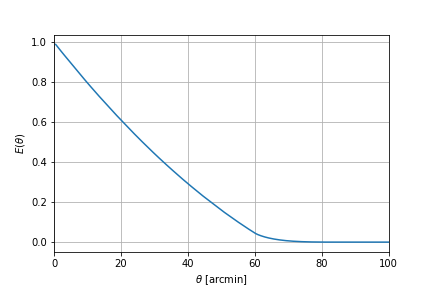
\includegraphics[width=0.5\textwidth]{images/eoftheta.png}
 \caption{Probability that a random pair of galaxies of distance $\theta$ lie in the same pointing.}
 \label{fig:eoftheta_lin}
 \end{figure}

We again parametrize the number density $N(\b \theta)=\la N \ra (1+n(\b \theta))$ and the weight $W(\b \theta)=1+w(\b \theta)$ and, as in \eqref{eq:defweightf}, interpret $n(\b \theta)$ as a locally constant function with average $\la n \ra = 0$. We can see that $\la n(\b 0)n(\b \theta)\ra = E(\theta)\la n(\b 0)n(\b 0)\ra \equiv E(\theta)\la n n \ra$ holds and get
 \begin{align}
\xi^{\text{obs}}_\pm(\theta) = & \frac{1 + 2\la nw \ra + E(\theta)\left[\la (n+w)^2\ra + 2 \la n^2 w\ra + 2\la nw^2\ra + \la n^2 w^2\ra \right]}{1+E(\theta)\la n^2\ra }\xi_\pm^{\rm const}(\theta) \\
\approx & \frac{1 + 2\la nw \ra + E(\theta)\left[\la (n+w)^2\ra \right]}{1+E(\theta)\la n^2\ra }\xi_\pm^{\rm const}(\theta)\, . \nonumber
 \label{eq:ffunct}
\end{align}
\todo{The formula for a cross-correlation of different bins is much longer, but follows the same principle. Maybe put it into the Appendix?}
We see that in addition to a modification of the correlation function due to the stronger shear signal in deeper pointings, we also get a scale-independent modification due to the correlation between depth and number density.

However, as a survey of constant depth is completely unrealistic, also the modelled correlation function will be subject to the same effect. If we assume the same redshift-distributions for galaxies as in the case of varying depth, and just assert that those changes are not correlated with position, we get 
\begin{equation}
\xi_\pm = (1+2\la nw\ra)\xi_\pm^{\rm const}\, .
\end{equation}
The ratio of modelled and observed correlation function thus becomes: \begin{align}
\frac{\xi_\pm}{\xi_\pm^{\rm obs}} = & \frac{\left(1+2\la nw\ra\left)\left(1+E(\theta)\la n^2\ra\right)\right.\right.}{1 + 2\la nw \ra + E(\theta)\left[\la (n+w)^2\ra + 2 \la n^2 w\ra + 2\la nw^2\ra + \la n^2 w^2\ra \right]} \\
\equiv & F(\theta) \, .
\end{align}
%It is interesting to note that $F(\theta)=1$ holds wherever $E(\theta)=0$, meaning that the correlation function is not affected for large angular scales. 
We shall later see that this approximation is valid for higher tomographic redshift bins $z\gtrsim 0.5$, but starts to break down at lower redshifts. 
\subsection{Using a semi-analytic Model}
The analysis of data from the Kilo-Degree Survey showed that the redshift-distribution of sources was highly correlated with the depth in the $r$-band. We thus chose to separate the survey into 10 percentiles, sorted by $r$-band depth, meaning that if a pointing had a worse depth than 90\% of the other pointings, it would belong to the first percentile, and so on. Now for each percentile $i$ and each tomographic redshift bin $z$ we can extract a weighted number density of galaxies $N_i(z)$ and, in case the pointing overlaps with a spectroscopic survey, a source redshift distribution $p_i(z)$. Using \eqref{eq:xipm-pkappa}, we can for each set of percentiles $i,j$ and redshift bins $z_1,z_2$ compute the shear correlation function $\xi_\pm[\theta,p_i(z_1),p_j(z_2)]$.\todo{Should we cite \textsc{nicaea} here?} When we compute the measured shear correlation function of a survey, we take the weighted average of tangential and cross shears of all pairs of galaxies (\citet{2017MNRAS.465.1454H} give a good overview for the process). If, for a single pair of galaxies, one galaxy lies in the $i$-th percentile of redshift bin $z_1$ and the second one lies in the $j$-th percentile of redshift bin $z_2$, then their contribution to the observed correlation function is, on average, $\xi_\pm[\theta,p_i(z_1),p_j(z_2)]$. This means that if we know each of those single correlation functions, we can reconstruct the total correlation function via a weighted average of the single functions. As an example, if we want to calculate the correlation function between tomographic bins $z_1$ and $z_2$ and pick a galaxy from bin $z_1$, the probability of this galaxy being in the $i$-th percentile of $z_1$ is proportional to $N_i(z_1)$. Now let the second galaxy be in bin $z_2$ and of distance $\theta$ to the first. If we imagine a thin annulus of radius $\theta$ around the first galaxy, then the number of galaxies in this annulus, that lie within the same pointing as the first galaxy, is proportional to $E(\theta)N_i(z_2)$, whereas the number of galaxies that lie in a different pointing is $[1-E(\theta)]\la N(z_2)\ra$, where $\la N(z_2)\ra$ is the average number density in redshift bin $z_2$. If the galaxy lies within a different pointing, the chances of it being in the $j$-th percentile are again just proportional to $N_j(z_2)$. We conclude that if we sum the single correlation functions $\xi_\pm[\theta,p_i(z_1),p_j(z_2)]$ according to these weightings, we can simulate the observed correlation function that accounts for the variation in optical depth via 
\begin{align}
\xi_{\pm,z_1,z_2}^{\rm obs}(\theta) = & \frac{1}{C}\sum_{i=1}^{10} N_i(z_1) \bigg\{ E(\theta) N_i(z_2) \xi_\pm\big[\theta,p_i(z_1),p_i(z_2)\big] + \la N(z_2)\ra\sum_{j=1}^{10}\frac{  N_j(z_2)}{\sum_k N_k(z_2)} \big[1-E(\theta)\big]\xi_\pm\big[\theta,p_i(z_1),p_j(z_2)\big]\bigg\} \nonumber \\
 = & \frac{1}{C}\sum_{i=1}^{10} N_i(z_1) \bigg\{ E(\theta) N_i(z_2) \xi_\pm\big[\theta,p_i(z_1),p_i(z_2)\big] + \sum_{j=1}^{10}\frac{1}{10} \big[1-E(\theta)\big] N_j(z_2)\xi_\pm\big[\theta,p_i(z_1),p_j(z_2)\big]\bigg\}\, ,
\label{eq:correctionfunction1}
\end{align}
with the normalization
\[
C = \sum_{i=1}^{10} N_i(z_1) \bigg[ E(\theta)  N_i(z_2) + \sum_{j=1}^{10} \frac{1}{10} \big[1-E(\theta)\big] N_j(z_2)\bigg]\,.
\]
A more mathematically rigorous derivation of this function can be found in Appendix \ref{sec:calc of xipm}.
If we want to compute this for all 5 redshift bins of the KiDSV-survey, this forces us to calculate 1265 correlation functions and add them, thus yielding potential numerical errors (apart from being computationally expensive). However, if we examine Equation \eqref{eq:lenseff}, we see that it is linear in its second argument, which in turn makes Equations \eqref{eq:pkappa-pdelta/lenseff} and \eqref{eq:xipm-pkappa} bilinear in their second and third arguments. This basically means that, instead of adding correlation functions, we can add their respective redshift distributions and compute the correlation function of that. As an example, the following equation holds: \[
N_j\xi_\pm[\theta,p_i,p_j]+N_k\xi_\pm[\theta,p_i,p_k] = (N_j+N_k)\,\xi_\pm\left[\theta,p_i,\frac{N_jp_j+N_kp_k}{N_j+N_k}\right]\, .
\]
Consequently, we can apply this to \eqref{eq:correctionfunction1}, yielding
\begin{equation}
\xi_{\pm,z_1,z_2}^{\rm obs}(\theta) = \frac{1}{C}\bigg\{ E(\theta)\sum_{i=1}^{10} N_i(z_1)N_i(z_2) \xi_\pm\big[\theta,p_i(z_1),p_i(z_2)\big] +\frac{1}{10}\big[1-E(\theta)\big]\xi_\pm\left[\theta,p(z_1),p(z_2)\right]N(z_1)N(z_2)\bigg\}\, .
\label{eq:correctionfunction2}
\end{equation}
Here, we defined the \textit{average redshift distribution} $p(z)$ and \textit{combined number density} $N(z)$ of tomographic bin $z$ as \[
p(z):= \frac{\sum_i N_i(z)p_i(z)}{\sum_i N_i(z)}\, , \qquad N(z):=\sum_i N_i(z)\, .
\]
\todo{Maybe label the $N(z)$ differently to avoid confusion with $\la N(z)\ra$?}
For each set of redshift bins we thus only have to compute eleven correlation functions, which reduces the number of functions to compute from 1275 to 165. We can see that for large distances $\theta$, such that $E(\theta)=0$ holds, we have $C=N(z_1)N(z_2)$ and thus \[
\xi_{\pm,z_1,z_2}^{\rm obs}(\theta) = \frac{1}{N(z_1)N(z_2)}\xi_\pm\left(\theta,n(z_1),n(z_2)\right)N(z_1)N(z_2) = \xi_{\pm,z_1,z_2}(\theta)\, ,
\]
so on large scales our observed correlation function agrees with the one that we would usually calculate.
